\documentclass[aspectratio=169]{beamer}
\usetheme{fdu}

% Packages
\usepackage{tikz} % plot in place
\usepackage{pgfplots} % rather include jpg/pdf
\pgfplotsset{compat=1.9}
\usepackage{diagbox} % diagbox for table
\usepackage[export]{adjustbox} % autofix for table
\usepackage[ruled]{algorithm2e}
\SetAlCapFnt{\tiny\sffamily} % setting fonts for algorithm caption
\usepackage{natbib} % bib cite package
\bibliographystyle{dinat} % set bib style
\setbeamercovered{transparent} % shadow words for overlay
\usepackage{listings}
\usepackage[UTF8]{ctex}
\setbeamertemplate{theorems}[numbered]

% Commands
\newcommand{\cA}{\mathcal{A}}
\newcommand{\cB}{\mathcal{B}}
\newcommand{\cC}{\mathcal{C}}
\newcommand{\cD}{\mathcal{D}}
\newcommand{\cE}{\mathcal{E}}
\newcommand{\cF}{\mathcal{F}}
\newcommand{\cG}{\mathcal{G}}
\newcommand{\cH}{\mathcal{H}}
\newcommand{\cI}{\mathcal{I}}
\newcommand{\cJ}{\mathcal{J}}
\newcommand{\cK}{\mathcal{K}}
\newcommand{\cL}{\mathcal{L}}
\newcommand{\cM}{\mathcal{M}}
\newcommand{\cN}{\mathcal{N}}
\newcommand{\cO}{\mathcal{O}}
\newcommand{\cP}{\mathcal{P}}
\newcommand{\cQ}{\mathcal{Q}}
\newcommand{\cR}{\mathcal{R}}
\newcommand{\cS}{\mathcal{S}}
\newcommand{\cT}{\mathcal{T}}
\newcommand{\cU}{\mathcal{U}}
\newcommand{\cV}{\mathcal{V}}
\newcommand{\cW}{\mathcal{W}}
\newcommand{\cX}{\mathcal{X}}
\newcommand{\cY}{\mathcal{Y}}
\newcommand{\cZ}{\mathcal{Z}}

\newcommand{\bA}{\mathbb{A}}
\newcommand{\bB}{\mathbb{B}}
\newcommand{\bC}{\mathbb{C}}
\newcommand{\bD}{\mathbb{D}}
\newcommand{\bE}{\mathbb{E}}
\newcommand{\bF}{\mathbb{F}}
\newcommand{\bG}{\mathbb{G}}
\newcommand{\bH}{\mathbb{H}}
\newcommand{\bI}{\mathbb{I}}
\newcommand{\bJ}{\mathbb{J}}
\newcommand{\bK}{\mathbb{K}}
\newcommand{\bL}{\mathbb{L}}
\newcommand{\bM}{\mathbb{M}}
\newcommand{\bN}{\mathbb{N}}
\newcommand{\bO}{\mathbb{O}}
\newcommand{\bP}{\mathbb{P}}
\newcommand{\bQ}{\mathbb{Q}}
\newcommand{\bR}{\mathbb{R}}
\newcommand{\bS}{\mathbb{S}}
\newcommand{\bT}{\mathbb{T}}
\newcommand{\bU}{\mathbb{U}}
\newcommand{\bV}{\mathbb{V}}
\newcommand{\bW}{\mathbb{W}}
\newcommand{\bX}{\mathbb{X}}
\newcommand{\bY}{\mathbb{Y}}
\newcommand{\bZ}{\mathbb{Z}}
\usepackage{hyperref}

%%% Titlepage information
\title[数据结构与算法导论]{商业决策平台的智能数据管理系统}
\author[卢羿舟]{\textbf{卢羿舟}}
\institute[复旦大学]{
    统计与数据科学系
}

% table of contents
\AtBeginSection[]{
    \begin{frame}<beamer>{目录}
    \tableofcontents[
        currentsection,
        currentsubsection, 
        hideothersubsections, 
        sectionstyle=show/shaded,
    ]
    \end{frame} 
}

\AtBeginSubsection[]{
  \begin{frame}{本节目录} % 或者就叫 "目录"
    \tableofcontents[currentsection, currentsubsection, subsectionstyle=show/shaded]
  \end{frame}
}

\begin{document}

\begin{frame}
  \titlepage
\end{frame}

\section{项目背景与目标}

\begin{frame}{项目背景}
    \begin{itemize}
        \item 在当今快速发展和竞争激烈的商业环境中,企业对于精准、高效的决策能力的需求日益增长。为了应对这一挑战,构建一个强大的商业决策平台显得尤为重要
        \item 你是一家新兴的“数据驱动商业决策平台”的员工,公司要求你帮助设计其底层数据处理模块。你需要设计一个系统支撑平台的智能化运行
    \end{itemize}
\end{frame}

\begin{frame}{问题回顾}
    该系统存储的数据包括
    \begin{itemize}
        \item 营销任务与任务之间的依赖关系
        \item 表示客户之间关系的加权有向图
        \item 商品数据
    \end{itemize}
    需要完成的功能包括
    \begin{itemize}
        \item 营销任务优先调度功能
        \item 客户网络与影响力传播分析
        \item 商品数据检索
    \end{itemize}
\end{frame}


\section{设计思路与功能分析}

\begin{frame}{整体规划}
    根据要求,将系统拆分成三个模块
    \begin{itemize}
        \item 营销任务优先调度模块
        \item 客户网络与影响力传播分析模块
        \item 商品数据检索模块
    \end{itemize}
\end{frame}

\subsection{营销任务优先调度模块}
\begin{frame}{模块功能拆解}
    目标:实现一个存储所有营销任务的数据结构,支持
    \begin{itemize}
        \item 对营销数据的增、删、改、查
        \item 根据任务之间的相互依赖优先执行优先级最高的任务
        \item 展示任务优先级最高的$k$个任务
    \end{itemize}
\end{frame}

\begin{frame}{核心数据结构与规划逻辑}
    \begin{itemize}
        \item 模块要求我们实现可以高效查找优先级最高的营销任务,同时还需要展示优先级最高的$k$个任务,优先队列可以很好的完成这个问题,因此该模块首选\textbf{优先队列}作为核心数据结构
        \item 在优先队列中,考虑且仅考虑当前不存在前置依赖的任务,存在前置依赖的任务会被移除出优先队列,而新增的不存在前置依赖的任务会被加入优先队列
    \end{itemize}
\end{frame}



\begin{frame}{任务依赖表示}
    为了考虑任务之间的前置依赖关系,我们需要实现一个有向图,规定
    \begin{align*}
        \text{前置任务} \longrightarrow \text{后置任务}
    \end{align*}
    为有向图的基本结构,同时
    为了避免出现相互依赖的问题,需要额外要求该有向图为有向无环图
\end{frame}

\begin{frame}{任务状态管理}
    为了更好的管理任务状态,考虑为任务附加一个属性$\mathtt{\_status}$,用来表示任务当前的状态。我们将任务的状态分成三类:
    \begin{itemize}
        \item $\mathtt{Pending}$
        \item $\mathtt{Ready}$
        \item $\mathtt{Complete}$
    \end{itemize}
    分别代表三种状态:该任务存在前置依赖,该任务不存在前置依赖与该任务已完成。
\end{frame}

\begin{frame}{任务ID设计}
    考虑可能会修改任务名,为了实现对任务的唯一识别,额外添加$\mathtt{\_task\_id}$属性,它满足
    \begin{itemize}
        \item 唯一性
        \item 不变性
    \end{itemize}
    在每一个营销任务对象被创建时就赋予其任务ID,设计格式为“时间戳-UUID\footnote{一个唯一的32位十六进制字符串}”,这样设计的好处是
    \begin{itemize}
        \item 在并发条件下ID不冲突
        \item ID存在一定的有序信息,方便检索和管理
    \end{itemize}
\end{frame}

\begin{frame}{Top-k功能设计}
    由于没有提前指定$k$的具体数量,所以无法直接在系统运行中提前规划大小为$k$的优先队列,为了实现这一功能,有两个设计思路
    \begin{enumerate}
        \item 每次调用时,优先队列连续弹出$k$个节点,记录信息后再插入优先队列恢复
        \item 复制一份优先队列,随后连续弹出$k$个节点后删除
    \end{enumerate}
    为了避免可能过高的空间复杂度,最终采用了方案1
\end{frame}

\begin{frame}{优先队列及任务状态管理逻辑}
    一个营销任务在其生命周期中,可能会经历以下状态改变:
    \begin{itemize}
        \item 初始化状态为\texttt{Ready}(由于不存在前置依赖)
        \item 由于被添加了前置依赖,状态由\texttt{Ready}变为\texttt{Pending}
        \item 由于前置依赖被完成或删除,状态由\texttt{Pending}变为\texttt{Ready}
        \item 处于优先队列队首被执行,状态由\texttt{Ready}变为\texttt{Complete}
    \end{itemize}
    对于每一次的状态改变,都会影响其本身和其后续任务在优先队列中的状态,此外,倘若修改处于\texttt{Ready}状态的任务优先级,也会影响其在优先队列中的位置,这需要我们能够高效调整优先队列,但。。。
\end{frame}

\begin{frame}{支持高效查找的优先队列设计}
    为了解决优先队列无法实现高效查找与删除的问题,该模块在以数组为基础的优先队列的基础上,额外维护一个字典,字典中的键值对为
    \begin{align*}
        \{\mathtt{task\_id}: \text{堆中索引}\}
    \end{align*}
    用于高效查找目标任务在堆中的位置,实现高效的更新与删除
\end{frame}


\begin{frame}{功能实现——\texttt{MarketingTask}类}
    \texttt{MarketingTask}类有以下属性:
    \begin{itemize}
        \item $\mathtt{\_task\_id}$
        \item $\mathtt{\_name}$
        \item $\mathtt{\_status}$
        \item $\mathtt{urgency}$
        \item $\mathtt{influence}$
        \item $\mathtt{\_priority}$
    \end{itemize}
    使用了\texttt{\_\_slots\_\_}命令来优化存储空间(因为这个类会被大量实例化),同时利用$\mathtt{@property}$和$\mathtt{setter}$来控制对这些私有变量的访问和修改,并在每次修改后自动更新优先级
\end{frame}

\begin{frame}{功能实现——\texttt{MarketingTask}类}
    此外,\texttt{MarketingTask}类还包含两个私有方法,用于更新任务的属性和状态
    \begin{itemize}
    \item $\mathtt{\_update\_details()}$\footnote{注意,由于美观性以及空间因素,在slides中所有出现的函数都默认不填写参数名和参数类型,详细的参数说明可以参考源代码注释。}:更新任务的紧急程度或者影响力,并更新优先级,如果某个参数为None,则不更新该属性,如果更新成功,则返回True,如果没有更新,则返回False
    \item $\mathtt{\_set\_status()}$:设置任务的状态
    \end{itemize}
\end{frame}

\begin{frame}{功能实现——$\mathtt{TaskDependencyGraph}$类}
    为了实现高效的查找节点相互之间的依赖关系,该类总共维护了两个字典,分别储正向依赖关系以及反向依赖关系,以及一个集合用于存储任务ID。其中正向依赖关系指的是从某个任务节点指向其他后续任务的映射,而反向依赖关系指的是某个任务节点被哪些任务前置影响的映射。它包含了以下图的基本方法
    \begin{itemize}
        \item $\mathtt{add\_task()}$:向图中添加一个任务节点
        \item $\mathtt{remove\_task()}$:从图中移除一个任务节点及其所有相关依赖, 并返回这个节点id
        \item $\mathtt{add\_dependency()}$:添加依赖关系:$\text{prerequisite\_id}$ -> $\text{dependent\_id}$,在添加前会进行环路检测
        \item $\mathtt{remove\_dependency()}$:移除依赖关系:$\text{prerequisite\_id}$ -> $\text{dependent\_id}$
        \item $\mathtt{get\_dependents()}$:获取直接依赖于$\text{task\_id}$的任务集合
        \item $\mathtt{get\_prerequisites()}$:获取$\text{task\_id}$的前置任务集合
        \item $\mathtt{has\_task()}$:检查任务是否存在于图中
        \item $\mathtt{get\_all\_tasks()}$:返回图中所有任务的列表
    \end{itemize}
\end{frame}

\begin{frame}{功能实现——$\mathtt{TaskDependencyGraph}$类}
    注意,由于我们要求图本身无环,所以在每次添加边的时候,需要对图进行环路检测。这个检测的原理是通过深度优先搜索寻找是否存在一条待添加边的反向通路,倘若存在,则不允许添加这条边,否则会导致图中出现环。这个深度优先搜索通过一个私有方法$\mathtt{\_has\_path()}$实现。这个方法通过列表模拟栈来实现了一个迭代式的深度优先搜索
\end{frame}

\begin{frame}{功能实现——$\mathtt{UpdatableMaxHeap}$类}
    与常规利用列表实现的最小堆不同的是,这个类额外维护了一个字典用于支持节点在列表中的索引查找,从而实现高效的查找和删除。由于堆中元素位置的变动完全由$\mathtt{\_swap()}$实现,所以只需要在该私有方法中加入更新索引字典的逻辑即可。下面展示公共接口列表
    \begin{itemize}
        \item $\mathtt{insert()}$:向堆中插入一个新任务,如果任务已存在,则更新优先级
        \item $\mathtt{peek\_max()}$:查看堆顶元素, 不移除
        \item $\mathtt{extract\_max()}$:移除并返回堆顶元素
        \item $\mathtt{is\_empty()}$:检查堆是否为空
        \item $\mathtt{update\_priority()}$:更新堆中已存在任务的优先级
        \item $\mathtt{delete()}$:从堆中删除指定任务ID的元素
        \item $\mathtt{get\_heap\_size()}$:返回堆中元素的数量
    \end{itemize}

\end{frame}

\begin{frame}{功能实现——$\mathtt{TaskManager}$类}
    这个类是营销任务优先调度模块的核心类,用于实现所有营销任务优先调度模块需要实现的功能。它维护了多个数据结构:
    \begin{itemize}
        \item $\mathtt{\_tasks}$:字典,任务ID到任务对象的映射
        \item $\mathtt{\_task\_graph}$:$\mathtt{TaskDependencyGraph}$类,储存任务之间的依赖关系
        \item $\mathtt{\_ready\_queue}$:$\mathtt{UpdatableMaxHeap}$类,储存所有状态为Ready的任务的优先队列
        \item $\mathtt{\_in\_degree}$:字典,状态为Pending的任务ID到其前置依赖数量的映射
    \end{itemize}
\end{frame}

\begin{frame}{功能实现——$\mathtt{TaskManager}$类}
这个类的公共接口
\begin{itemize}
    \item $\mathtt{add\_task()}$:往任务管理器中添加一个任务
    \item $\mathtt{add\_dependency()}$:添加一个任务间的依赖关系,如果添加的依赖会导致后继任务不再ready,则需要将其从ready队列中移除
    \item $\mathtt{remove\_dependency()}$:移除一个已经存在的依赖关系,如果移除成功且导致后继任务的状态变为ready,则更新ready队列
    \item $\mathtt{mark\_task\_as\_completed()}$:将指定任务标记为已完成,同时更新其后续任务的入度字典
    \item $\mathtt{execute\_next\_highest\_priority\_task()}$:从ready队列中提取优先级最高的任务,并执行
    \item $\mathtt{get\_top\_k\_ready\_tasks()}$:查看当前ready队列中的优先级最高的k个任务
    \item $\mathtt{update\_task\_info()}$:更新现有的任务信息
    \item $\mathtt{delete\_task()}$:从系统中彻底删除一个任务及其所有相关依赖
\end{itemize}
\end{frame}

\subsection{客户网络与影响力传播分析模块}
\begin{frame}{模块功能拆解}
    这个模块需要实现对客户关系网络的分析。首先我们定义所有客户与相互的影响关系被储存在一个有向图(这里的图可以有环)中,每个节点均表示一个客户。他们之间的影响关系如下
\begin{align*}
    \text{客户}A \overset{0.8}{\longrightarrow} \text{客户}B
\end{align*}
代表客户A可以直接影响客户B,而边权代表客户A对客户B的影响程度,这个数值的取值范围为了分析方便被限制在了$(0,1]$,数值越大代表影响程度越深,从而依靠这种关系来构建整个有向图。在这个模块中总共有两个分析任务:
\begin{enumerate}
    \item 客户重要性评价
    \item 寻找每一位客户所能影响到的所有客户
\end{enumerate}
\end{frame}

\begin{frame}{客户重要性评价}
    为了识别客户关系网中最重要的节点,客户网络与影响力传播分析模块实现了两个判断节点重要性的算法
    \begin{enumerate}
        \item 度中心性
        \item PageRank
    \end{enumerate}
\end{frame}

\begin{frame}{度中心性}
    要衡量一个图中节点的重要性,一个很直观的方法就是看他的入边和出边有多少。这类似于评价一个交通枢纽的重要程度,它能够连接起越多的路,一般而言就越重要。这个评价指标就被称为加权度中心性(\textbf{W}eighted \textbf{D}egree \textbf{C}entrality),加权度中心性越高,代表节点的重要性越高。在有向赋权图中,这个指标进一步变为加权入度中心性(WIDC)和加权出度中心性(WODC),这是为了区分不同边的性质和不同的边权,具体计算方式如下
\begin{align*}
    WIDC(o) = \sum_{u \in in(o)} w(u, o),\quad WODC(o) = \sum_{u\in out(o)} w(o, u),
\end{align*}
其中$in(o)$和$out(o)$分别代表节点$o$的所有入射节点和出射节点。

\end{frame}

\begin{frame}{度中心性的问题}
    度中心性存在以下问题
    \begin{itemize}
        \item 仅考虑相邻节点之间的影响
        \item 所有节点对影响力的贡献是等价的
    \end{itemize}
    然而,在我们的例子中,客户A如果能通过客户B而对C有影响,那么客户A的重要程度也应该能传导到对客户C的重要程度的评价上。如果一个客户能同时影响更多的客户,它的影响力应该和只能影响很少客户的影响力有所不同
\end{frame}

\begin{frame}{PageRank}
    PageRank~\citep{Page1999ThePC}最开始被用于评价网页重要性,其核心思想基于这样一种直观的理念:一个网页的重要性取决于指向它的其他网页的数量和质量。
    简单来说,PageRank 算法模拟了一个在互联网上随机冲浪的用户。用户从一个随机的网页开始,然后不断地点击页面上的链接。一个网页被访问的概率越高,那么这个网页就被认为越重要。
\end{frame}

\begin{frame}{影响力范围分析}
    为了综合考虑两个节点之间的距离和边权重对影响程度的影响,引入路径影响力概念,具体而言,对于节点$u$和节点$v$,设这两个节点之间的路径集合为$\mathcal{L}$,则这两点之间的路径影响力定义为
\begin{align*}
    IF(u, v) = \max_{l\in \mathcal{L}} \prod_{o, o^\prime \in l} w(o, o^\prime),
\end{align*}
即为路径途径所有边的边权乘积中的最大值。由于之前限制了边权的取值范围为$(0, 1]$,所以最终的路径影响力取值范围也应该为$(0, 1]$,且影响力值随着路径延长单调递减,我们可以很容易设置一个截断阈值来获得在一定范围和影响力内的客户影响力集合。
\end{frame}

\begin{frame}{功能实现——$\mathtt{CustomerGraph}$类}
    该类为一个允许环路的有向赋权图,使用邻接列表来存储,该数据结构存在以下公共接口
    \begin{itemize}
    \item $\mathtt{add\_customer()}$:向图中添加一个新客户(节点) 如果客户已存在,则不执行任何操作
    \item $\mathtt{get\_all\_customers()}$:返回图中所有客户名称的列表
    \item $\mathtt{add\_influence()}$:在两个客户之间添加一条有向的影响力关系(边) 如果 'from\_customer' 或 'to\_customer' 不在图中,会先将它们添加进来
    \item $\mathtt{get\_direct\_influencees()}$:获取一个客户直接影响的所有其他客户及其对应的影响力权重
    \item $\mathtt{get\_influence\_weight()}$:获取从 from\_customer 到 to\_customer 的直接影响力权重 
\end{itemize}
\end{frame}

\begin{frame}{功能实现——算法}
    基于$\mathtt{CustomerGraph}$类,实现了以下四个算法:
\begin{itemize}
    \item $\mathtt{calculate\_weighted\_out\_degree\_centrality()}$
    \item $\mathtt{calculate\_weighted\_in\_degree\_centrality()}$
    \item $\mathtt{calculate\_pagerank()}$
    \item $\mathtt{analyze\_all\_customer\_influence\_nodes()}$
\end{itemize}
\end{frame}

\subsection{商品数据检索模块}
\begin{frame}{模块功能拆解}
    在这个模块中,我们需要维护一个管理所有商品的结构,需要实现的功能如下:
    \begin{itemize}
        \item 高效插入、删除、更改商品信息和搜索
        \item 搜索任意价格范围内的所有商品
        \item 根据商品名称前缀进行前缀搜索
    \end{itemize}
    同时需要考虑过多的商品无法一次性加载进入内存查找,需要对外存查找进行优化
\end{frame}

\begin{frame}{平衡二叉搜索树的外存低效}
    想象在一个很厚的有序字典(数据)中找一个词,字典非常厚以至于分成了上万本存放在图书馆(硬盘)里,你的书桌(内存)无法放下所有的字典,一次只能取一本查找,所以可能要频繁去书架上找下一次搜索到的字典(多次磁盘I/O操作),每次只能拿回来一本书,而去书架取书太慢了,所以会造成查找低效
\end{frame}

\begin{frame}{B+树}
    \begin{columns}
        \begin{column}{0.6\textwidth}
            为了提高外存搜索效率,有两个可以优化的方法
            \begin{itemize}
                \item 降低去书架找书的次数
                \item 相近的词一定连续地存放在同一个字典中(外存中的数据存储一般是离散的)
            \end{itemize}
            B+树优化了这两个方向,进而实现了高效的外存查找
        \end{column}
        \begin{column}{0.4\textwidth}
            \begin{figure}[t]
                \begin{center}
                \centerline{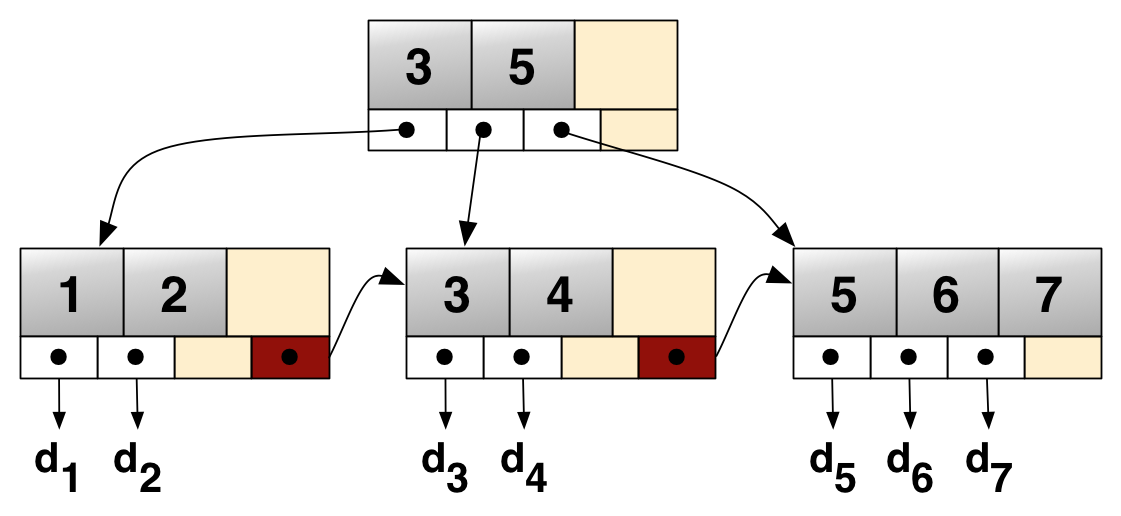
\includegraphics[width=0.9\columnwidth]{resources/Bplustree.png}}
                \caption{B+树的基本结构}
                \label{fig: bplustree}
                \end{center}
            \end{figure}
        \end{column}
    \end{columns}
\end{frame}

\begin{frame}{前缀搜索}
    \begin{columns}
        \begin{column}{0.6\textwidth}
            Trie是一种天然支持前缀搜索的树,其每一个节点都代表字符串中的某一位字符,因此如果想要实现前缀搜索,只需要搜索到前缀末尾的那个字符对应的节点,然后遍历即可。
        \end{column}
        \begin{column}{0.4\textwidth}
            \begin{figure}[t]
                \begin{center}
                \centerline{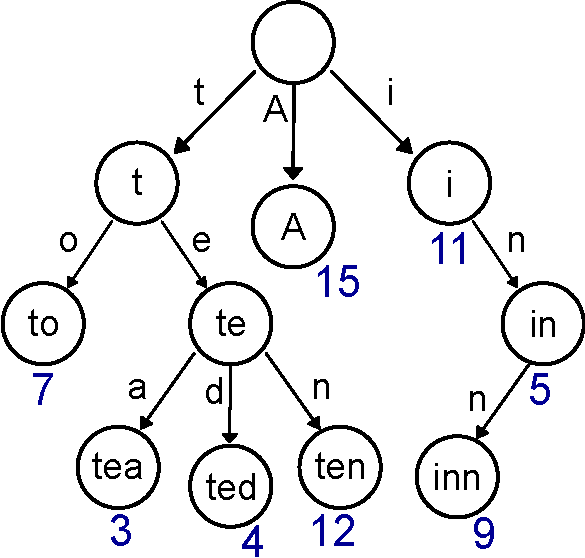
\includegraphics[width=0.6\columnwidth]{resources/Trie_example-crop.pdf}}
                \caption{一个保存了8个键的trie结构,"A", "to", "tea", "ted", "ten", "i", "in", "inn"}
                \label{fig: trie example}
                \end{center}
            \end{figure}
        \end{column}
    \end{columns}
\end{frame}

\begin{frame}{商品ID设计}
    与此前\texttt{MarketingTask}相同,我们需要一个对商品对象的唯一标识,设计格式为“PROD-时间戳-UUID”,目的与此前一样,且可以与营销任务的ID做明显的区分
\end{frame}

\begin{frame}{数据存储逻辑设计}
    回顾我们总结的模块功能,我们需要至少实现通过价格和商品名进行查找,然而商品价格和商品名都有可能发生更改和重复。这在数据存储中是极为低效的,意味着我们需要存储两套商品对象的副本,出现大量的存储空间浪费,为此,在该模块借用数据库设计理念,作出如下设计
    \begin{itemize}
        \item \textbf{主键}:为商品对象的唯一ID,可以通过主键查找商品对象
        \item \textbf{次键}:包括商品名和商品价格等,可以通过次键查询对应的商品ID
    \end{itemize}
    这样实现了
    \begin{enumerate}
        \item 优化存储空间
        \item 提高数据一致性和维护效率
    \end{enumerate}
\end{frame}

\begin{frame}{功能实现——\texttt{Product}类}
    与\texttt{MarketingTask}类类似,\texttt{Product}类通过\texttt{@property}和setter来规定对其属性的访问和修改操作,同时对于这种会大量实例化的类,通过\texttt{\_\_slots\_\_}进行存储优化,其包含如下属性
    \begin{itemize}
        \item \texttt{\_product\_id}
        \item \texttt{name}
        \item \texttt{price}
        \item \texttt{heat}
    \end{itemize}
\end{frame}

\begin{frame}{功能实现——B+树}
    由于模块中需要有两种不同的B+树,一种键和值是一一对应的关系(ID-Product对象),一种一个键可以对应一系列值(价格-ID)。两种B+树在搜索、插入、删除等逻辑上存在细微差别,因此,首先定义了\texttt{BaseBPlusTree}作为基类,规定了B+树的一系列底层操作,模块中使用的两种B+树均继承自这个基类。关于B+树,总共实现了以下四个类
    \begin{itemize}
        \item \texttt{BPlusTreeNode}:B+树节点类,定义内部节点和叶节点的行为
        \item \texttt{BaseBPlusTree}:B+树基类,定义B+树的底层操作
        \item \texttt{BPlusTreeProducts}:用于存储(价格-ID)对,支持范围查找
        \item \texttt{BPlusTreeID}:用于存储(ID-Product对象)对
    \end{itemize}
\end{frame}

\begin{frame}{功能实现——Trie树}
    第二个次键是商品名,用来通过商品名前缀或者全程来搜索对应商品的逻辑。这部分实现了以下两个类
    \begin{itemize}
        \item \texttt{TrieNode}:节点类,标记该节点是否为单词末尾,若是,存放对应商品ID
        \item \texttt{ProductPrefixTrie}:实现了一个Trie树,支持插入、删除和前缀匹配
    \end{itemize}
    与标准Trie树不同的是,普通Trie树在删除时仅仅删除节点上的标记,这会导致大量的存储空间浪费,为此,在实现Trie树的delete方法时,额外实现了一个基于回溯的节点删除逻辑,回收不再用于索引商品名的冗余节点
\end{frame}

\begin{frame}{功能实现——\texttt{ProductManager}类}
    这个类用于实现该模块的所有功能,包括
    \begin{itemize}
        \item 添加、删除、更新商品信息
        \item 通过ID精确搜索商品
        \item 通过价格进行模糊搜索和范围搜索
        \item 通过前缀进行模糊搜索(仅返回k个热度最高的商品)
        \item 通过全称进行搜索
    \end{itemize}
    其使用\texttt{BPlusTreeID}存储ID作为主键,使用\texttt{BPlusTreeProducts}存储价格作为次键,使用\texttt{ProductPrefixTrie}存储名称作为次键,实现高效的索引
\end{frame}

\section{改进思路}
\begin{frame}{关于营销任务优先调度模块}
    在考虑营销任务前置依赖的优先调度时,该模块目前仅仅考虑在不存在前置依赖的任务中进行优先度排序,从中选择优先度最高的执行。然而,在实际环境中,可能存在某个前置任务虽然不紧急,但是其后置任务十分紧急的情况,而当前的算法无法捕捉这种后继任务的重要性。

    \textbf{解决方案}:由于规定了营销任务之间的依赖图不能有环,而任何一个有向无环图可以通过若干条不相交的路径进行路径覆盖,因此考虑将依赖图拆分成多条路径,对于每一条路径进行整体的优先级排序。
\end{frame}

\begin{frame}{路径优先级}
    定义路径优先级,首先定义一个衰减因子\footnote{本质是一个惩罚项,越靠后的高优先级任务需要提前完成的代价越大。}$\gamma$,则路径中某个节点$o$对路径优先级的影响力可以计算为
    \begin{align*}
        IF(o) = \gamma^k \text{priority}(o),
    \end{align*}
    其中$k$为路径起点到节点$o$的步数,衰减因子可以由任务的时效性决定,时效性越强的任务,$\gamma$越接近于$1$。通过对路径优先级进行排序,来决定优先执行哪一条路径的第一个任务。当有任务被完成时,重新计算路径优先级。
\end{frame}

\begin{frame}{关于客户网络与影响力传播分析模块}
    这部分功能主要有以下三个改进方向
    \begin{enumerate}
        \item 当前仅仅采用了度中心性和PageRank来评价节点重要性,但是并未有一个综合的统计分析,未来可以继续添加其他的评价指标,然后构建统计模型进行综合分析
        \item 关于最小影响力阈值,对于不同结构不同节点数量的图,理想的阈值应该不一样,现在主要依靠经验制定,后续可以使用一些指标进行自适应计算
        \item 当前处理图数据的主要思路是Offline的,但是在真实业务场景中,数据往往是Online的,可以通过缓存已有的路径信息来提升运行效率,降低计算开销
    \end{enumerate}
\end{frame}

\begin{frame}{关于商品数据检索模块}
    当前使用Trie树进行前缀匹配,然而Trie树在外存的效率并不高,后续可以考虑将B+树和Trie树结合起来,使用B+树的每一个叶节点存放一个Trie树的方式,来提升前缀匹配效率
\end{frame}

\begin{frame}{源代码}
    \url{https://github.com/FDULeolu/data_structure_pj}
    \\
    感兴趣的同学可以帮忙点点Star,谢谢!
\end{frame}


\begin{frame}{References}
    \tiny
    \bibliography{reference}
\end{frame}

\end{document}